\documentclass[tikz]{standalone}
\usepackage{tikz, pgfplots}
\usetikzlibrary{svg.path}
\pgfplotsset{compat=1.16}
\usepgfplotslibrary{fillbetween}
\begin{document}
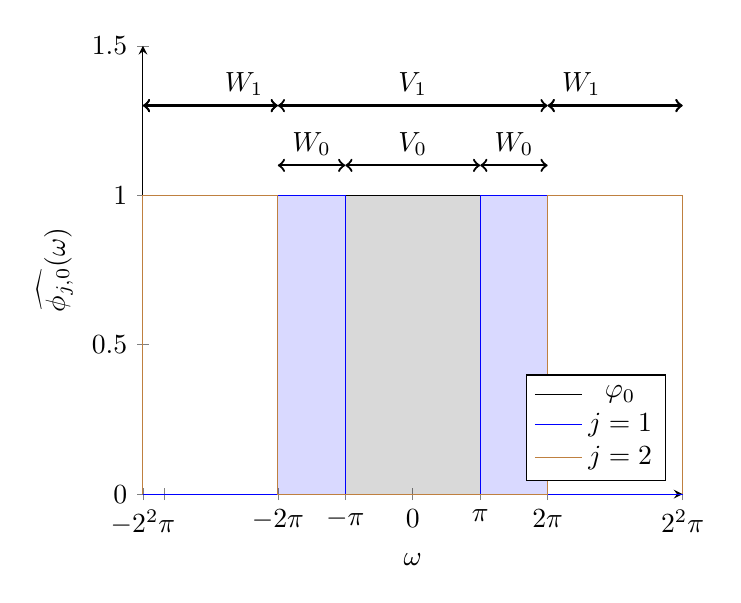
\begin{tikzpicture}[baseline]
	\begin{axis}[
		clip=false,
		xlabel =$\omega$,
		ylabel = $\widehat{\phi_{j, 0}}(\omega)$,
		axis x line = bottom,
		axis y line = left,
		ymax=1.5,
		%x=3cm,
		legend entries={$\varphi_0$,$j=1$, $j=2$},
		legend pos = south east,
		xtick={-2^2*pi+1, -2^2*pi, -2*pi, -pi, 0, pi, 2*pi, 2^2*pi, 2^2*pi+1},	
		xticklabels={$$, $-2^2\pi$, $-2\pi$,$ -\pi$, $0$, $\pi$,$2\pi$, $2^2\pi$, $$},
		trig format plots = rad]
		\addplot[	color=black, 
				name path=phi
			] coordinates{
					(-2^2*pi, 0)
					(-pi, 0)
					(-pi, 1)
					(pi, 1)
					(pi, 0)
					(2^2*pi, 0)
					};
		\draw[<->, black, thick] (-pi, 1.1) to (pi, 1.1);
		\draw[<->, black, thick] (-2*pi, 1.1) to (-pi, 1.1);
		\draw[<->, black, thick] (pi, 1.1) to (2*pi, 1.1);
		\draw[<->, black, thick] (-2^2*pi, 1.3) to (-2*pi, 1.3);
		\draw[<->, black, thick] (2*pi, 1.3) to (2^2*pi, 1.3);
		\draw[<->, black, thick] (-2*pi, 1.3) to (2*pi, 1.3);
		\draw[<->, black, thick] (-2^2*pi, 1.3) to (-2*pi, 1.3);
		\draw[<->, black, thick] (2*pi, 1.3) to (2^2*pi, 1.3);
		\filldraw (0,1.1) node[anchor=south]{$V_0$};
		\filldraw (-3*pi/2,1.1) node[anchor=south]{$W_0$};
		\filldraw (3*pi/2,1.1) node[anchor=south]{$W_0$};
		\filldraw (- pi -3*pi/2,1.3) node[anchor=south]{$W_1$};
		\filldraw (pi+3*pi/2,1.3) node[anchor=south]{$W_1$};
		\filldraw (0,1.3) node[anchor=south]{$V_1$};
			\addplot[	blue,
				name path=psi1
				]  coordinates{
					(-2^2*pi, 0)
					(-2*pi, 0)
					(-2*pi, 1)
					(-pi, 1)
					(-pi, 0)
					(pi, 0)
					(pi, 1)
					(2*pi, 1)
					(2*pi, 0)
					(2^2*pi, 0)				
					};


		\addplot[	brown, 
				domain = -pi:pi,
				]  coordinates{
					(-2^2*pi, 0)
					(-2^2*pi, 0)
					(-2^2*pi, 1)
					(-2*pi, 1)
					(-2*pi, 0)
					(2*pi, 0)
					(2*pi, 1)
					(2^2*pi, 1)
					(2^2*pi, 0)
					(2^2*pi, 0)				
					}; 
	\path[draw = none,name path=supphi, black, opacity=0] 
			(-pi,0) 
			(pi, 0);
				
		\addplot[draw=none, dashed, opacity=0.15] fill between[
			of = phi and supphi,
			%soft clip={domain=-pi/2,pi/2},
			];
		\path[draw = none,name path=suppsi1, brown, opacity=0] 
			(-2*pi,0)
			(-pi,0)

			(pi, 0)
			(2*pi, 0);
				
		\addplot[color=blue, dashed, opacity=0.15] fill between[
			of = psi1 and suppsi1,
			%soft clip={domain=-pi/2,pi/2},
			];






	\end{axis}
\end{tikzpicture}
\end{document}

